\documentclass{article}

\usepackage{amsfonts}
\usepackage{graphicx}
\usepackage{amssymb}
\usepackage{amsmath}
\usepackage{listings}
\usepackage{hyperref}


\DeclareMathOperator{\sech}{sech}
\newcommand{\NN}{\mathbb{N}}
\newcommand{\RR}{\mathbb{R}}
\newcommand{\QQ}{\mathbb{Q}}
\newcommand{\ZZ}{\mathbb{Z}}
\newcommand{\dV}{\;\mathrm{d}V}
\newcommand{\dA}{\;\mathrm{d}A}
\newcommand{\dx}{\;\mathrm{d}x}
\newcommand{\dy}{\;\mathrm{d}y}
\newcommand{\dz}{\;\mathrm{d}z}
\newcommand{\cA}{\mathcal{A}}
\newcommand{\Bb}{\mathcal{B}}
\newcommand{\Ww}{\mathcal{W}}
\newcommand{\Dd}{\mathcal{D}}
\newcommand{\Ss}{\mathcal{S}}
\newcommand{\Ee}{\mathcal{E}}
\DeclareMathOperator{\im}{im}

\tolerance=1
\emergencystretch=\maxdimen
\hyphenpenalty=10000
\hbadness=10000

\setlength\parindent{18pt}

\begin{document}

\Large{Lincoln Sand}


\textbf{G1.}

\textbf{128.1}:

Find where to place the fulcrum in a lever of length 10 m so that a weight of
14 kg at one end will balance a weight of 10 kg at the other.

Let's denote the following:

$L$ as the total length of the lever, which is 10 m.

$F_1$ as the force exerted by the 14 kg weight.

$F_2$ as the force exerted by the 10 kg weight.

$x$ as the distance from the 14 kg weight to the fulcrum.

$L - x$ as the distance from the fulcrum to the 10 kg weight.

The principle of moments gives us:

$F_1 \cdot x = F_2 \cdot (L - x)$

Solving for $x$ gives approximately $x = 4.17$ m.


\textbf{128.11}:

Use calculus to prove Archimedes' result that the area of a parabolic segment
is four-thirds of the area of the inscribed triangle.

Let's first find the area of the parabolic segment:

\[A_{\text{parabolic segment}} = \int_{-d}^{d} a x^2 dx = \frac{2}{3} a d^3\]

The area of the triangle formed by the intersection of the tangent lines of the endpoints
of the line with the parabola gives:

\[T_1 = \frac{1}{2} \cdot 2 d \cdot a d^2 = a d^3\]

But the inscribed triangle is always exactly half of this triangle.

So, $T_2 = \frac{1}{2} T_1 = \frac{1}{2} a d^3$.

Notice that $\frac{4}{3} \cdot \frac{1}{2} a d^3 = \frac{2}{3} a d^3$.

Thus, we have shown the theorem.

You can look at the following diagram for clarification regarding the two triangles.

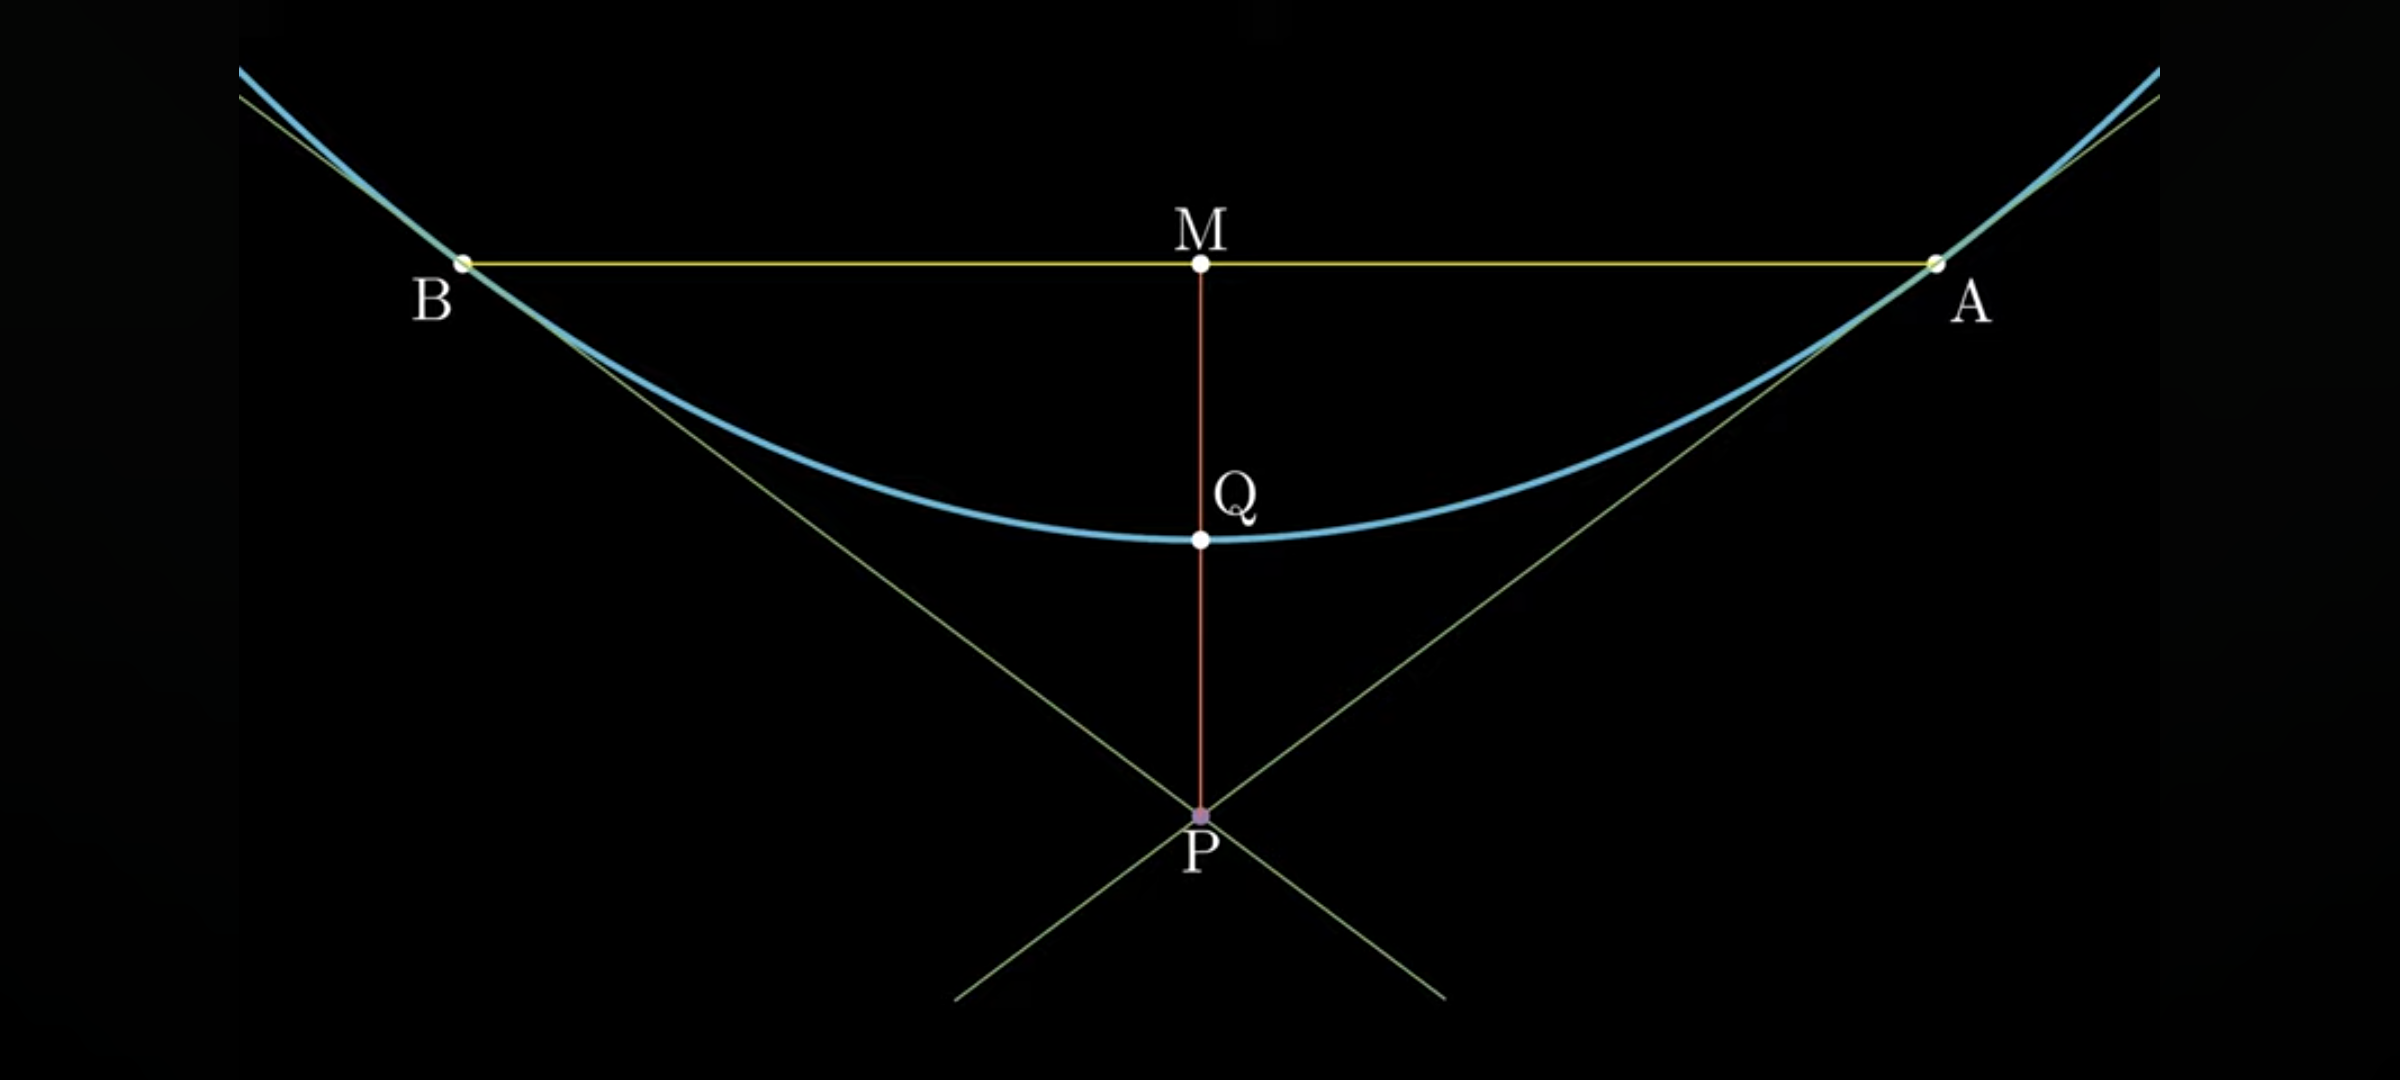
\includegraphics[width=\linewidth]{quadrature_parabola}


\textbf{G2.}

Show that if "a | bc" and gcd(a, b) = 1, then "a | c".

Assume that a | bc. This means there exists an integer k such that bc = ak.

Assume gcd(a, b) = 1. This means a and b have no common prime factors.

By Bezout's identity, $\exists$ integers x and y such that $ax + by = 1$.

Multiply both sides by c to get $axc + byc = c$.

Since a divides bc and bc = ak, replace bc with ak to get $axc + aky = c$.

Factor a to get $a(xc + ky) = c$.

This shows that c is a multiple of a since $xc + ky$ is an integer.

Thus, a | c.

\textbf{G3.}

Here is how Menaechchmus constructed the parabola as the locus of points $P = \{(x,y)\}$.
Given points A, O, and X on line such that 'a' is the distance AO and 'x' is the distance
OX. Let L be a perpendicular line through O. For each x, construct a circle whose diameter
is AX. Then 'y' is the distance from O to the intersection point of L with the circle.
Show that Menaechchmus' construction yields the parabola. Show that the parabola passes
through the point (a, a).

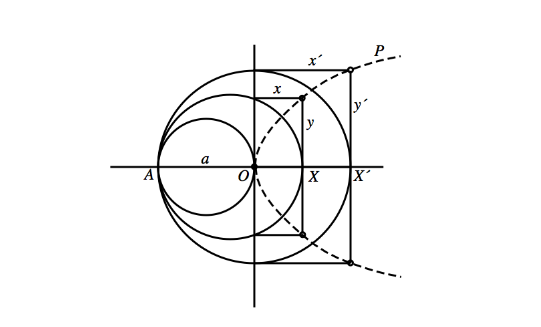
\includegraphics[width=\linewidth]{parabola_construction}

AO = a

OX = x

AX = a + x

Note that, because the circle of radius G is half of the large circle,
then, OX' is a since the large circle is perfectly bisected by L.

Because of the fact of how the largest circle is bounded by $x'$ and $y'$,
this means that $x' = y' = OX'$.
We know that $x' = y'$ because O is the midpoint and thus, O to the boundary
of the circle in any direction is the radius a.
And bith x' and y' measure the distance from O to the boundaries of the circle
along the x and y axes respectively. 

And because we know that $OX'$ is a, and that $P$ is $(x', y')$,
then $P = (a, a)$.


\textbf{G4.}


Show that any two tetrahedra with the same base and height can be approximated arbitrarily closely by the same prisms, differently stacked, as in the provided figure. Deduce that two tetrahedra with the same base and height have equal volume.

HINT: You may assume that the apex of the tetrahedron is directly over the base, which yields to a simpler analysis. Be careful! You have to take into account how skew your tetrahedron is. If T and T' are the tetrahedra and $S_n$ and ${S'}_n$ are the approximating stacks of prisms with n levels, we have volumes $V(S_n) = V({S'}_n)$ but we need to establish for Eudoxus's exhaustion method, that for any positive number $\epsilon > 0$, the stacks and tetrahedra are close enough so that both $|V(T) - V(S_N)| < \frac{\epsilon}{2}$ and $|V(T') - V({S'}_n)| < \frac{\epsilon}{2}$ for some n large enough, depending on $\epsilon$. You will need to compare inner and outer approximations for this. A problem occurs if the stacks spill outside the tetrahedron, as in the right tetrahedron in the diagram. We conclude from the triangle inequality, that for any $\epsilon > 0$, there is an n such that:
\[|V(T) - V(T')| = |V(T) - V(S_n) + V(S_n) - V({S'}_n) + V({S'}_n) - V(T')|\]
\[\leq |V(T) - V(S_n)| + |V(S_n) - V({S'}_n) + |V({S'}_n) - V(T')|\]
\[< \frac{\epsilon}{2} + 0 + \frac{\epsilon}{2} = \epsilon\]
Since $\epsilon$ may be any positive number no matter how small, $V(T) = V(T')$.

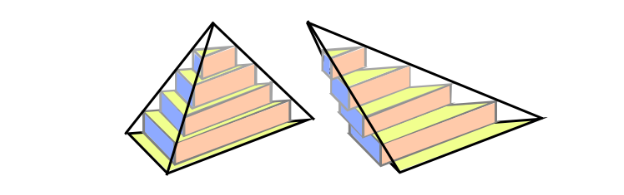
\includegraphics[width=\linewidth]{tetrahedra}

Divide each tetrahedron into a stack of prisms that have the same base area
and whose combined height is equal to the height of the tetrahedra.
As n, the number of prisms increases, the prisms become thinner, and the sum
of their volume approaches the volume of the tetrahedron.

Since the base area and height are the same of each prism for both $S_n$
and ${S'}_n$, the volume of each corresponding pair of prisms is the same,
thus $V(S_n) = V({S'}_n)$ for any n.

For any positive number $\epsilon$, we can find an n large enough such that
the difference between the volume of the tetrahedron and the volume of the stack
of prisms is less than $\frac{\epsilon}{2}$ for each tetrahedron. This is the case
since as we increase n, the prisms better approximate the shape of the tetrahedron
and the unoccupied space inside decreases.

Since the volume of the stack of prisms is the same for both $S_n$ and ${S'}_n$,
we can say that the difference in volume between $T$ and $T'$ must be less than
$\epsilon$. This is because the volume of T is within $\frac{\epsilon}{2}$
of $V(S_n)$ and the volume of T' is within $\frac{\epsilon}{2}$ of $V({S'}_n)$.

Thus, since $\epsilon$ can be made arbitrarily small, the volumes of $T$
and $T'$ must be equal. Otherwise, we would have a minimum
positive difference between their volumes, which contradicts the results
from above.

Therefore, we conclude that two tetrahedra with the same base and height have
equal volumes. The skewness of the tetrahedra does not affect this result.
The spilling of prisms outside the skewed tetrahedron does not occur
in the actual approximation, as each prism fits exactly within the tetrahedron'S
boundaries when sliced horizontally.


\end{document}
